\documentclass[12pt, twoside]{report}

%% comment this line for handouts. Uncomment for lecture notes
%\newcommand{\lectureNoteMode}{}

\raggedbottom

\usepackage{color, xifthen, amsthm, amssymb, amsmath, tikz, pgfplots}
\pgfplotsset{compat=1.18}
\usetikzlibrary{backgrounds}
\usepackage[letterpaper, margin=1in]{geometry}
\usepackage{multicol}
\usepackage{fourier}  %don't use txfonts b/c the sf doesn't look good

\usepackage{enumitem}
\setlist{topsep=-\parskip/2}


\setlength{\parindent}{0pt}
\setlength{\parskip}{\baselineskip}


\usepackage{mdframed} % makes better frames around examples (eg pagebreak allowed)
  % from mdframed package. used for examples
\newmdenv[
  skipabove=10pt,%\topsep,
  skipbelow=10pt,%\topsep
  ]{allrules}

\usepackage{tcolorbox} % for colored boxes


\usepackage{subfigure}
\usepackage{hyperref}
\hypersetup{colorlinks, urlcolor=red, linkcolor=.} %color urls, but not interal refs
\usepackage{graphicx, floatflt}
\graphicspath{{./figs/}{../figs/}}
\DeclareGraphicsExtensions{.png,.jpg,.pdf}

\usepackage{wrapfig}  %useful for wrapping text around pictures or tables
		      %though it doesn't do a great job inside my example boxes


\definecolor{defbod}{rgb}{.8,.8,.8}     \definecolor{defhead}{rgb}{.7,.1,.1}
\definecolor{thmbod}{rgb}{.8,.8,.8}     \definecolor{thmhead}{rgb}{.1,.1,.9}
\definecolor{factbod}{rgb}{1,1,1}    \definecolor{facthead}{rgb}{.1,.7,.1}
\definecolor{exbod}{rgb}{1,1,1}         \definecolor{exhead}{rgb}{0,.3,0}
\definecolor{soltext}{rgb}{.2,.2,.5}
\definecolor{notebod}{rgb}{.9,.9,.9}    \definecolor{notehead}{rgb}{.1,.1,.7}

\newcommand{\defn}[1]{
 \noindent \colorbox{defbod}{\begin{minipage}{.95\linewidth}
 \hspace{-12pt}\colorbox{defhead}{\sf\color{white} Definition}
 #1
 \end{minipage} } \medskip
 }
\newcommand{\dt}[1]{\textcolor{defhead}{\bfseries #1}}

\newcommand{\thrm}[1]{
 \noindent \colorbox{thmbod}{\begin{minipage}{.95\linewidth}
 \hspace{-12pt}\colorbox{thmhead}{\sf\color{white}Theorem}
 #1
 \end{minipage} } \medskip
 }
\newcommand{\coro}[1]{
 \noindent \colorbox{thmbod}{\begin{minipage}{.95\linewidth}
 \hspace{-12pt}\colorbox{thmhead}{\sf\color{white}Corollary}
 #1
 \end{minipage} } \medskip
 }
\newcommand{\fact}[1]{  %%%% !! note this different from calcnotes
 \noindent \begin{allrules}
 #1
 \end{allrules} \medskip
 }

\newcommand{\note}[1]{
	\noindent \colorbox{notebod}{\begin{minipage}{.95\textwidth}
			\hspace{-12pt}\colorbox{notehead}{\sf\color{white}NOTE}
			#1
	\end{minipage} } \medskip
}


% making the example thing with a line down the left.
\newmdenv[
rightline=false,
bottomline=false,
skipabove=0pt,%\topsep,
skipbelow=0pt,%\topsep
]{siderules}

\newcommand{\ex}[1]{
  \noindent \begin{siderules}
    \textcolor{exhead}{\sf Example}
    #1
  \end{siderules} 
  \medskip
}




%%%%%%%%%% set it up so that these are not displayed when 
%%%%%%%%%% printing notes for students?  or for overhead?
\newcommand{\exsol}[1]{
  {\color{soltext} #1}
}

\newcommand{\mynonumsect}[2][]{
 \cleardoublepage
 \section*{#1\hskip16pt #2}
 \addcontentsline{toc}{section}{#1 #2}
}

\newcommand{\myhead}[1]{
\par%\vskip\baselineskip
\noindent
{\large\bf #1}
}

%%%%%%%%%%%%%%%%%%%%%%%%
% symbol shortcuts

\newcommand{\nice}{\displaystyle}
\newcommand{\eqq}{\ensuremath \stackrel{?}{=}}
\newcommand{\R}{\ensuremath{\mathbb{R}}}




% %%%%%%%%%%%%%%%%%%%%%%%%
% %
% % Creating handouts vs notes
% %% If you use the line below before loading this file then it will be set up for
% %% lecture notes.  Default is for handouts
% %%
% %% \newcommand{\lectureNoteMode}{}
% %%
% %% do not uncomment here, just add the line to the file where you input this one.
% \ifthenelse{\not\isundefined\lectureNoteMode}
% { % lecture notes 
%   \newcommand{\Hvskip}[1]{}
%   \newcommand{\Hvfill}{}
%   \newcommand{\Hpbreak}{}  % pagebreaks for handouts
%   \newcommand{\Npbreak}{\vfill\pagebreak} % pagebreaks for printable notes
%   \newcommand{\Nonly}[1]{#1} % shows in notes, not in handouts
%   \newcommand{\mycleardoublepage}{\cleardoublepage}

%   \newcommand{\ex}[1]{
%    \noindent \begin{allrules}
%     \textcolor{exhead}{\sf Example}\par
%     #1
%     \end{allrules} \medskip
%   }

% } 
% { 
% %% Handout mode 
% %% this section sets it up with smaller margins, and blank spots for writing solns to examples
%   %%%%%%%%%%%%%%%%%%%%%%%%%%%%%%%%%%%%%%%%%%
%   %change frame around examples
%   % from mdframed package
%   \newmdenv[
%   rightline=false,
%   bottomline=false,
%   skipabove=0pt,%\topsep,
%   skipbelow=0pt,%\topsep
%   ]{siderules}
  
%   \newcommand{\ex}[1]{
%     \noindent \begin{siderules}
%       \textcolor{exhead}{\sf Example}
%       #1
%     \end{siderules} 
%     \medskip
%   }
  
%   %
%   %%%%%%%%%%%%%%%%%%%%%%%%%%%%%%%%%%%%%%%%%%
  
%   % don't show solutions for examples
%   \renewcommand{\exsol}[1]{}
  
%   %used for making blank space in handouts. eg: \vs2
%   \newcommand{\Hvskip}[1]{\vskip#1in\null}
%   \newcommand{\Hvfill}{\vfill} %vfill only in handouts mode
%   \newcommand{\Hpbreak}{\pagebreak} % pagebreaks for handouts
%   \newcommand{\Npbreak}{} % pagebreaks for printable notes
%   \newcommand{\Nonly}[1]{} % shows in printable, not in handouts
%   \newcommand{\mycleardoublepage}{\newpage} % don't need blank pages if not printing
  
%   % don't really need margins since not printing.
%   \geometry{margin=0.75in}

%   \renewcommand{\mynonumsect}[2][]{
%     \mycleardoublepage
%     \section*{#1\hskip16pt Handout: #2}
%     \addcontentsline{toc}{section}{#1 #2}
%   }

% } 





\setlength{\parindent}{0pt}

\setcounter{chapter}{1}
\begin{document}

\mynonumsect[0.0]{Coordinate Points}

\textbf{Goal:} To plot and read Coordinate Points off of a Cartesian Plane





\fact{
	\myhead{Cartesian Plane:}
	\begin{itemize}
		\item The Cartesian Plane is named after the French mathematician Rene Descartes.
		\item It is also called the \dt{Cartesian Coordinate System}.
		\item It consists of two lines (or axes, each called an axis) and a center point.
			\begin{itemize}
				\item The \dt{$x$-axis} is the horizontal line.
				\item The \dt{$y$-axis} is the vertical line.
				\item The \dt{Origin} is the intersection of the axes.
			\end{itemize}
		\item The axes divide the plane into four \dt{quadrants}.
		\item Each point corresponds to an \dt{Ordered Pair} of two real valued numbers, denoted $(x,y)$.  
			\begin{itemize}
				\item The $x$ and $y$ values tell the distance from the center Origin point.
				\item Since the Origin does not have any distance in either direction, its coordinate is $(0,0)$.
			\end{itemize}	
	\end{itemize}
}


\begin{center}
	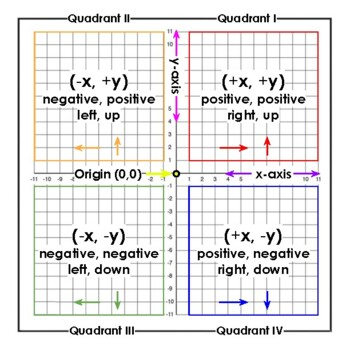
\includegraphics[alt={Coordinate plane showing the x-axis, y-axis, origin, and the four quadrants.}, width=4.25in]{105_0.0_coordinates2.jpg}
\end{center}



\pagebreak

\fact{ 
	\myhead{Plotting Coordinate Points:}
	\begin{itemize}
		\item Start at the ORIGIN $(0,0)$.
		\item Move LEFT/RIGHT the number of units as indicated by the $x$-coordinate.
			\begin{enumerate}
				\item Move to the RIGHT if your $x$-value is \emph{Positive}.
				\item Move to the LEFT if your $x$-value is \emph{Negative}.
			\end{enumerate}
		\item Move UP/DOWN the number of units as indicated by the $y$-coordinate.
		\begin{enumerate}
			\item Move UP if your $y$-value is \emph{Positive}.
			\item Move DOWN if your $y$-value is \emph{Negative}.
		\end{enumerate}
	\end{itemize}

\hskip1.5in 
\Large{You CRAWL before you stand TALL!}
}

\begin{center}
	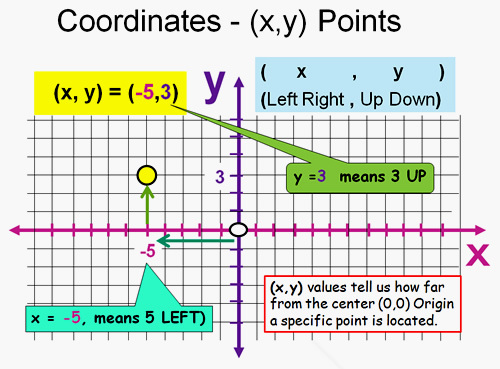
\includegraphics[alt={Coordinate plane example showing how to plot ordered pairs by moving horizontally along x and vertically along y from the origin.}, width=4.5in]{105_0.0_coordinates4.jpg} \\
	%https://bpshal.weebly.com/coordinate-plane-graphing.html
	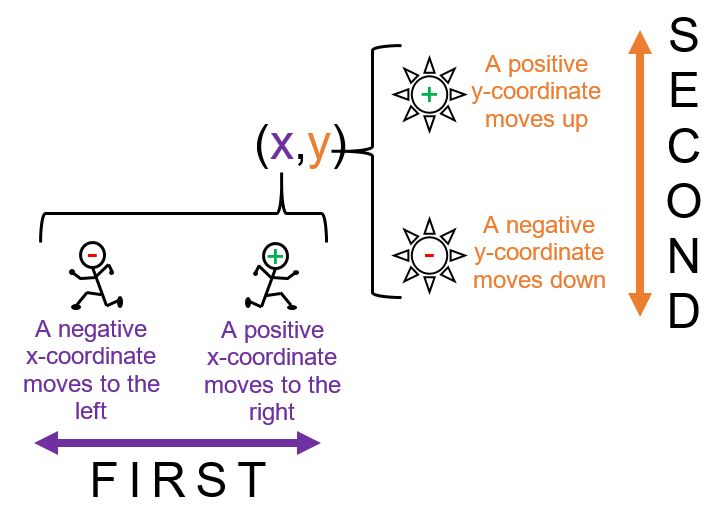
\includegraphics[alt={Worked example of a coordinate grid with labeled points plotted in different locations.}, width=3.25in]{105_0.0_coordinates3.jpg} \hfill 
	%https://www.exploremathindemand.com/the-coordinate-plane-notes.html
	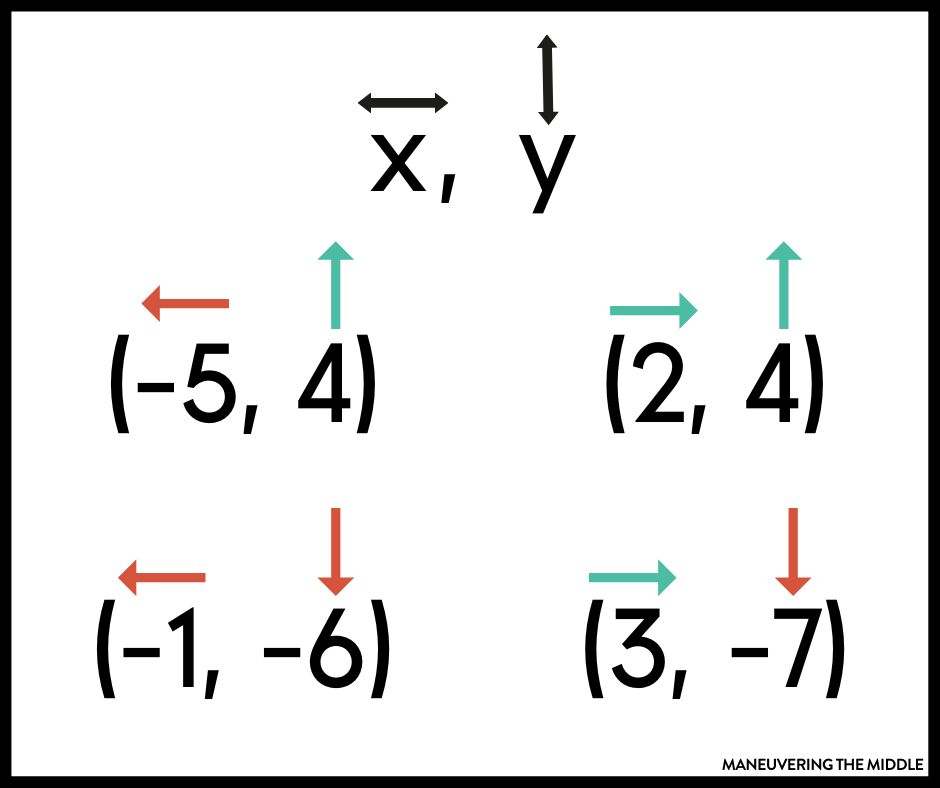
\includegraphics[alt={Coordinate plane activity graphic with example points used for plotting practice.}, width=2.5in]{105_0.0_coordinates5.jpg}
	%https://www.maneuveringthemiddle.com/coordinate-plane-activities-to-try/
\end{center}


\pagebreak

\myhead{Practice!}

\begin{enumerate}
	\item Plot and label the following points on the coordinate plane.
	%https://www.teacherspayteachers.com/Product/Graphing-in-the-Coordinate-Plane-GUIDED-NOTES-5074968
	\begin{multicols}{4}
			\begin{enumerate}
			\item $A(4,3)$
			\item $B(-4,3)$
			\item $C(0,5)$
			\item $D(3,0)$
			\item $E(-2,-1)$
			\item $F(2,-4)$
			\item $G(-4,0)$
			\item $H(0,-4)$
		\end{enumerate}
		
	\end{multicols}
	
	\begin{center}
		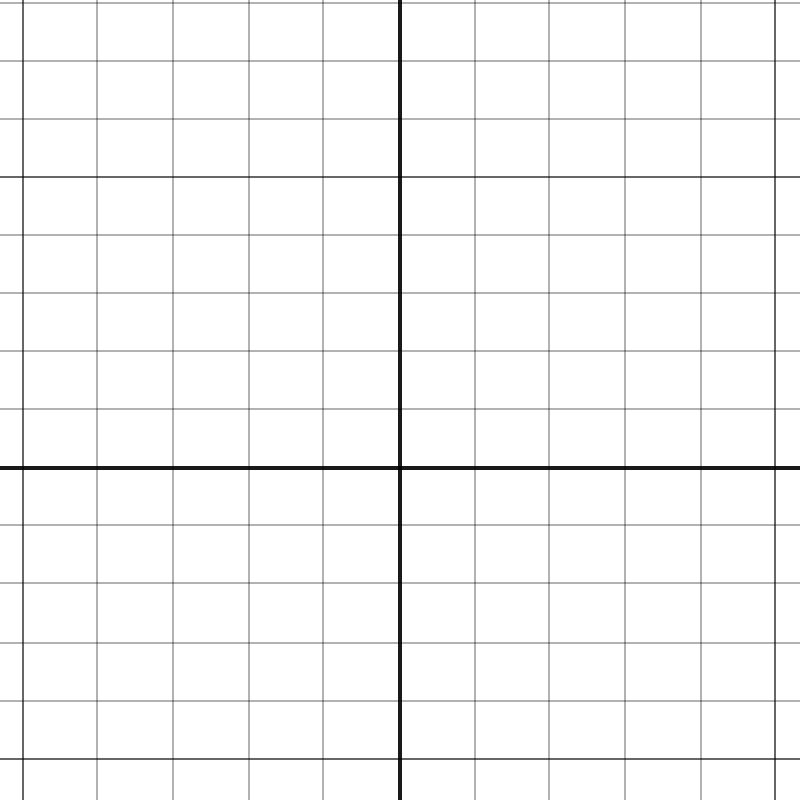
\includegraphics[alt={Blank graph paper for plotting and labeling points on a coordinate plane.}, width=4in]{105_graphpaper.jpg}
	\end{center}
	
	
	\item Describe the quadrant or axis in which each point lies: \\
		\begin{enumerate}
			\item The points that lie in Quadrant I are: \hrulefill \\
			\item The points that lie in Quadrant II are: \hrulefill \\
			\item The points that lie in Quadrant III are: \hrulefill \\
			\item The points that lie in Quadrant IV are: \hrulefill \\
			\item The points that lie on the $x$-axis are: \hrulefill \\
			\item The points that lie on the $y$-axis are: \hrulefill
		\end{enumerate}
		
\pagebreak

	\item Supply and Demand Scenario: A small market studies the relationship between price and quantity sold.  The owner collects the following data:
	\begin{itemize}
		\item At $\$10$, the market sold 100 units.
		\item At $\$15$, the market sold 80 units.
		\item At $\$20$, the market sold 60 units.
		\item At $\$25$, the market sold 40 units.
	\end{itemize}	
	
		\begin{enumerate}
		\item Write each data point as a coordinate and plot on the coordinate plane. \\
		Label the $x$-axis as Price ($\$$) and the $y$-axis as Quantity Sold (units). \\
		\item Using the graph, what can you conclude about Demand with respect to Price? \\ \\
		\phantom{.} \hrulefill
	\end{enumerate}
		
		
		\begin{center}
%			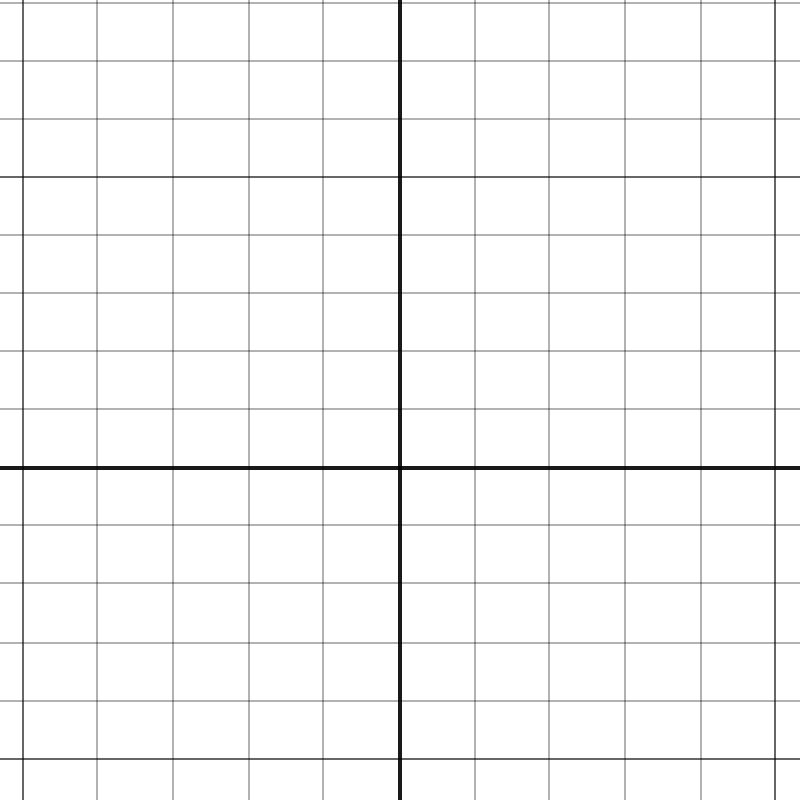
\includegraphics[width=4in]{105_graphpaper.jpg}
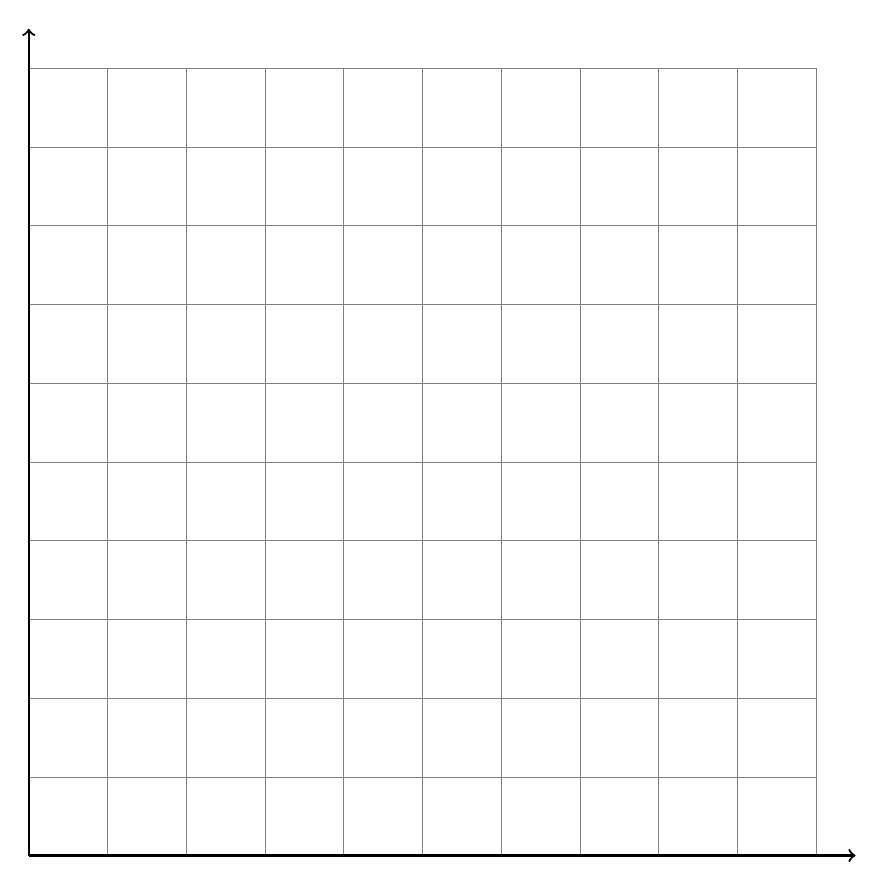
\begin{tikzpicture}[scale=1]
	% Draw gray grid
	\draw[step=1cm,gray,very thin] (0,0) grid (10,10);
	
	% Draw x and y axes with arrows
	\draw[thick,->] (0,0) -- (10.5,0); % x-axis with arrow
	\draw[thick,->] (0,0) -- (0,10.5); % y-axis with arrow
\end{tikzpicture}

		\end{center}
		
		\begin{center}
			
\includegraphics[alt={Illustration related to Rene Descartes, included as a decorative image near the end of the lesson.}, width=4in]{105_0.0_coordinates1.jpg} \hfill 
			%https://quantumawareness.net/2023/03/11/meditating-with-rene-descartes-part-2/
		\end{center}
\end{enumerate}





\pagebreak

\begin{center}
	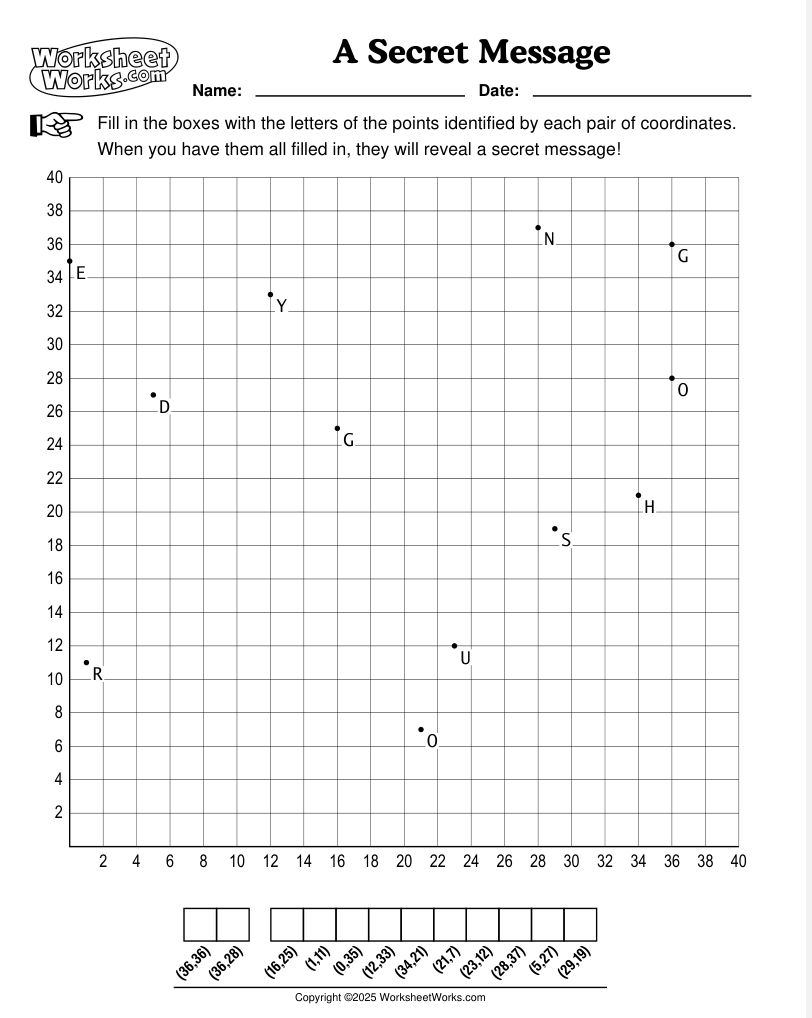
\includegraphics[alt={Large coordinate plane diagram showing axes and plotted example points for review.}, width=6.5in]{105_0.0_coordinates6.jpg}
\end{center}

\end{document}
